\chapter{Results}\label{chap:results}

\section{Dataset}

We use a dataset from a data center of Baidu Inc.
It is a subset of the dataset used in \cite{Zhu13}.

The reason for using only a subset is that due to GDPR limitations we do not have access to the Chinese website where the dataset is hosted.
So, we use a subset from it that is available on Kaggle \footnote{Dataset available at \url{https://www.kaggle.com/datasets/drtycoon/hdds-dataset-baidu-inc}}.

Despite only having access to a subset, our dataset includes all the 433 failing disks on the original dataset, which is the most important aspect since in general this is the class with a much smaller amount of members.
It also includes 5317 healthy disks.

In the dataset, for each disk a sample is taken every hour.
The observation period is of 7 days for healthy disks and 20 days for failing ones.
In total there are more than a million SMART attribute samples.

The model of every disk is the same.
This model makes available 12 different SMART attributes.
In the dataset they are already normalized to be between -1 and 1.
We can compute a change rate corresponding to each attribute, which allows us to obtain up to 24 different features.

\section{Binary Models}

We first perform the experiments using the classical approach of binary classification.
As stated on \ref{sec:software}, the full list of hyperparameters is made available in our repository.
The results for each model are listed on Table \ref{table:results_binary}.

\begin{table}
  \begin{center}
    \begin{tabular}{|c|c|c|c|c|}
      \hline
    Model & FAR(\%) & FDR(\%) & TIA(h) & TIA SD(h) \\
    \hline
    BPNN & 1.82 & 98.46 & 355.8 & 146.8 \\
    RNN & 1.63 & 99.23 & 369.3 & 137.7 \\
    LSTM & 1.57 & 97.69 & 358.7 & 144.1 \\
    Classification Tree & 1.13 & 99.23 & 353.7 & 147.8 \\
    Regression Tree & 1.13 & 99.23 & 334.9 & 154.3 \\
    \hline
    \end{tabular}
    \caption[Results Binary Models]{Results for binary models with default hyperparameters}
    \label{table:results_binary}
  \end{center}
\end{table}

We also show the distribution of the time in advance with which the failing disks were correctly detected in the histograms of Figures \ref{fig:tia_binary_network} and \ref{fig:tia_binary_tree}.

\begin{figure}
\begin{center}
  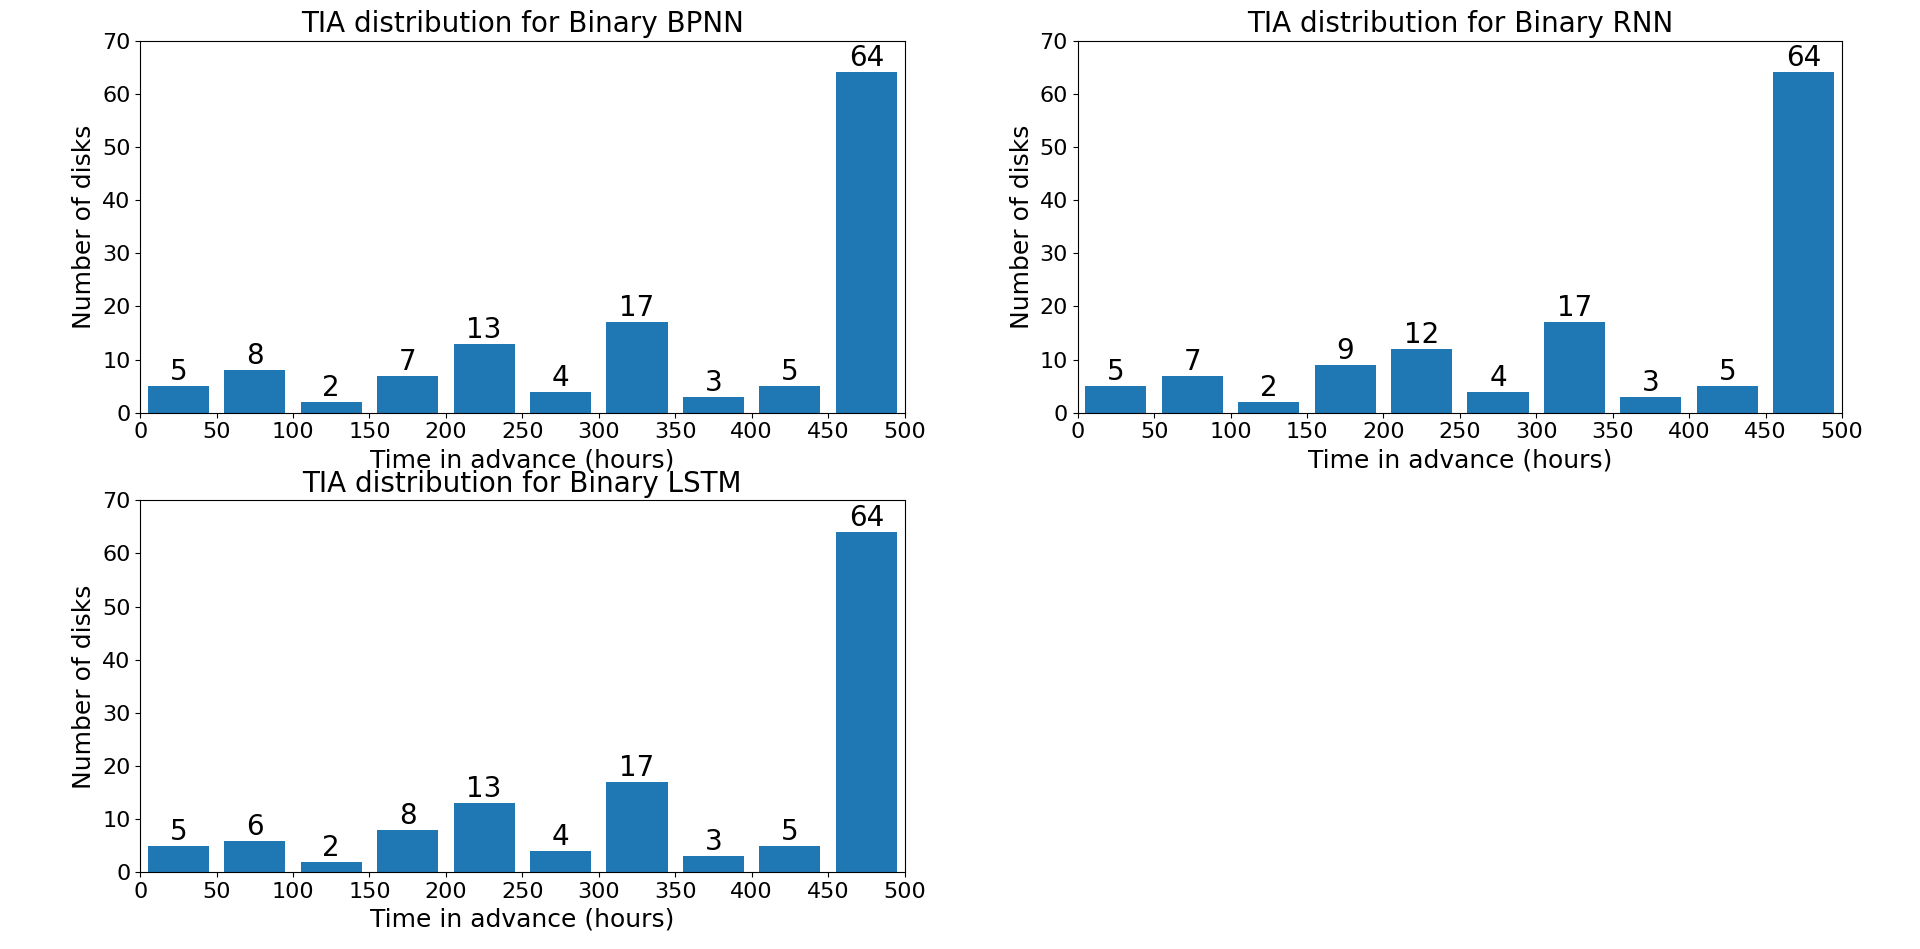
\includegraphics[width=1.0\linewidth]{TIA_Binary_Networks.png}
  \caption[TIA for binary networks]{Time In Advance distribution for binary networks}
  \label{fig:tia_binary_network}
\end{center}
\end{figure}

\begin{figure}
\begin{center}
  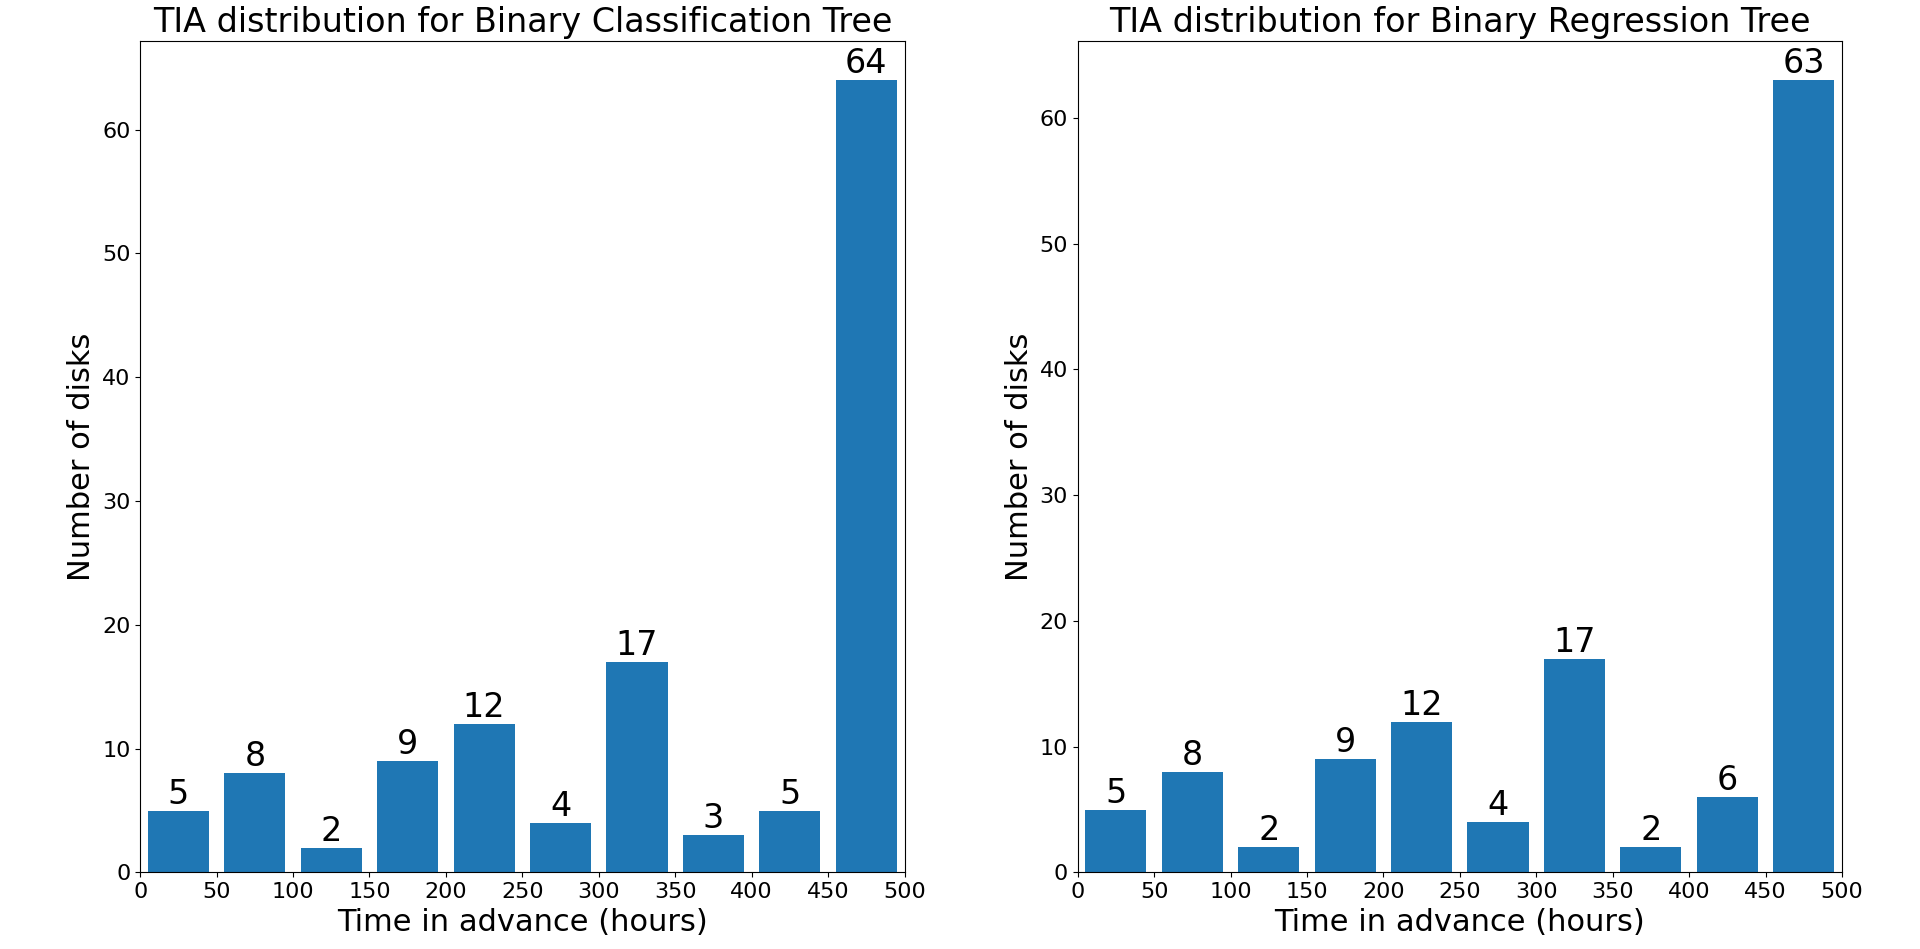
\includegraphics[width=0.9\linewidth]{TIA_Binary_Trees.png}
  \caption[TIA for binary decision trees]{Time In Advance distribution for binary decision trees}
  \label{fig:tia_binary_tree}
\end{center}
\end{figure}

The analysis we can make of these results is firstly that the three network models behave similarly.
For these models, the RNN is the one that presents the best performance, since its FDR is the highest among the three, and it obtains only a slightly higher FAR than the LSTM.

The two decision tree models perform better than any of the network based models since they have a smaller FDR than any of the BPNN, RNN and LSTM while achieving the maximum FDR found over the three models.
The classification tree is able to obtain a higher TIA with a smaller standard deviation than the regression tree, so it can be considered marginally better.

The distribution of the TIA for the different models signals that all of them are capable of detecting signals of problems hundreds of hours in advance
In practical terms, this means that the people responsible for managing the data centers will have plenty of time to swap the failing disks and prevent any data loss or disruption of service.

The smallest value of the TIA for correctly identified disks in the test set over every model was 19 hours.
This implies that no rushing is needed when a failure is predicted.
The main risk lies instead on the failures that have not been detected.

The capacity of such models to be highly sensitive to failing disks in order to detect problems much before they occur while keeping an FAR below 2\% proves that all of them are powerful methods to tackle the problem at hand.

Concerning the time to train and test the models, we have the decision trees being the fastest ones to train, taking 2 minutes on average.
The BPNN also takes a very short time, around 4 minutes.

The RNN and LSTM take a little longer: on average 8 minutes.
This is due to the fact that these are time sensitive models and therefore the samples must be evaluated in order.
This reduces the capabilities of the model to perform tasks in parallel.

All experiments have been performed on an ordinary desktop computer, with an AMD Ryzen 5 5560U CPU.
No GPU acceleration was needed.

We can compare our results to other experiments performed on the same dataset in \cite{Zhu13}, in which an FAR of 1.14\% and an FDR of 97.69\% obtained.
In their experiments, the model used was a BPNN.

Our decision tree models outperform theirs, since ours have achieved a smaller FAR and a higher FDR.
For the neural network models, we mostly obtained a better FDR but a worse FDR than them, even though the difference between the two experiments are not the same.
So there is a tradeoff between the two metrics which is to be expected.

The advantage of our approach is that we can directly compare the performance of different models without introducing bias due to different datasets or different preprocessing steps.

On the next few pages we will describe the impact of the feature selection algorithms as well as how the voting process can improve the results.
Finally, we will show that the inclusion of the change rates of the SMART attributes improves the performance of every model.

\subsection{Feature Selection Algorithms}

We have trained our different models using the different feature selection algorithms described on Subsection \ref{subsec:feature_selection}.
We still keep the same hyperparameters as the experiments performed on the last section, with the only modifications being on the feature count that was set to 15, to better observe if the algorithm really ranked higher the critical features,  and, of course, on the feature selection algorithm.
The results are displayed on Figure \ref{fig:fs_binary}.

\begin{figure}
\begin{center}
  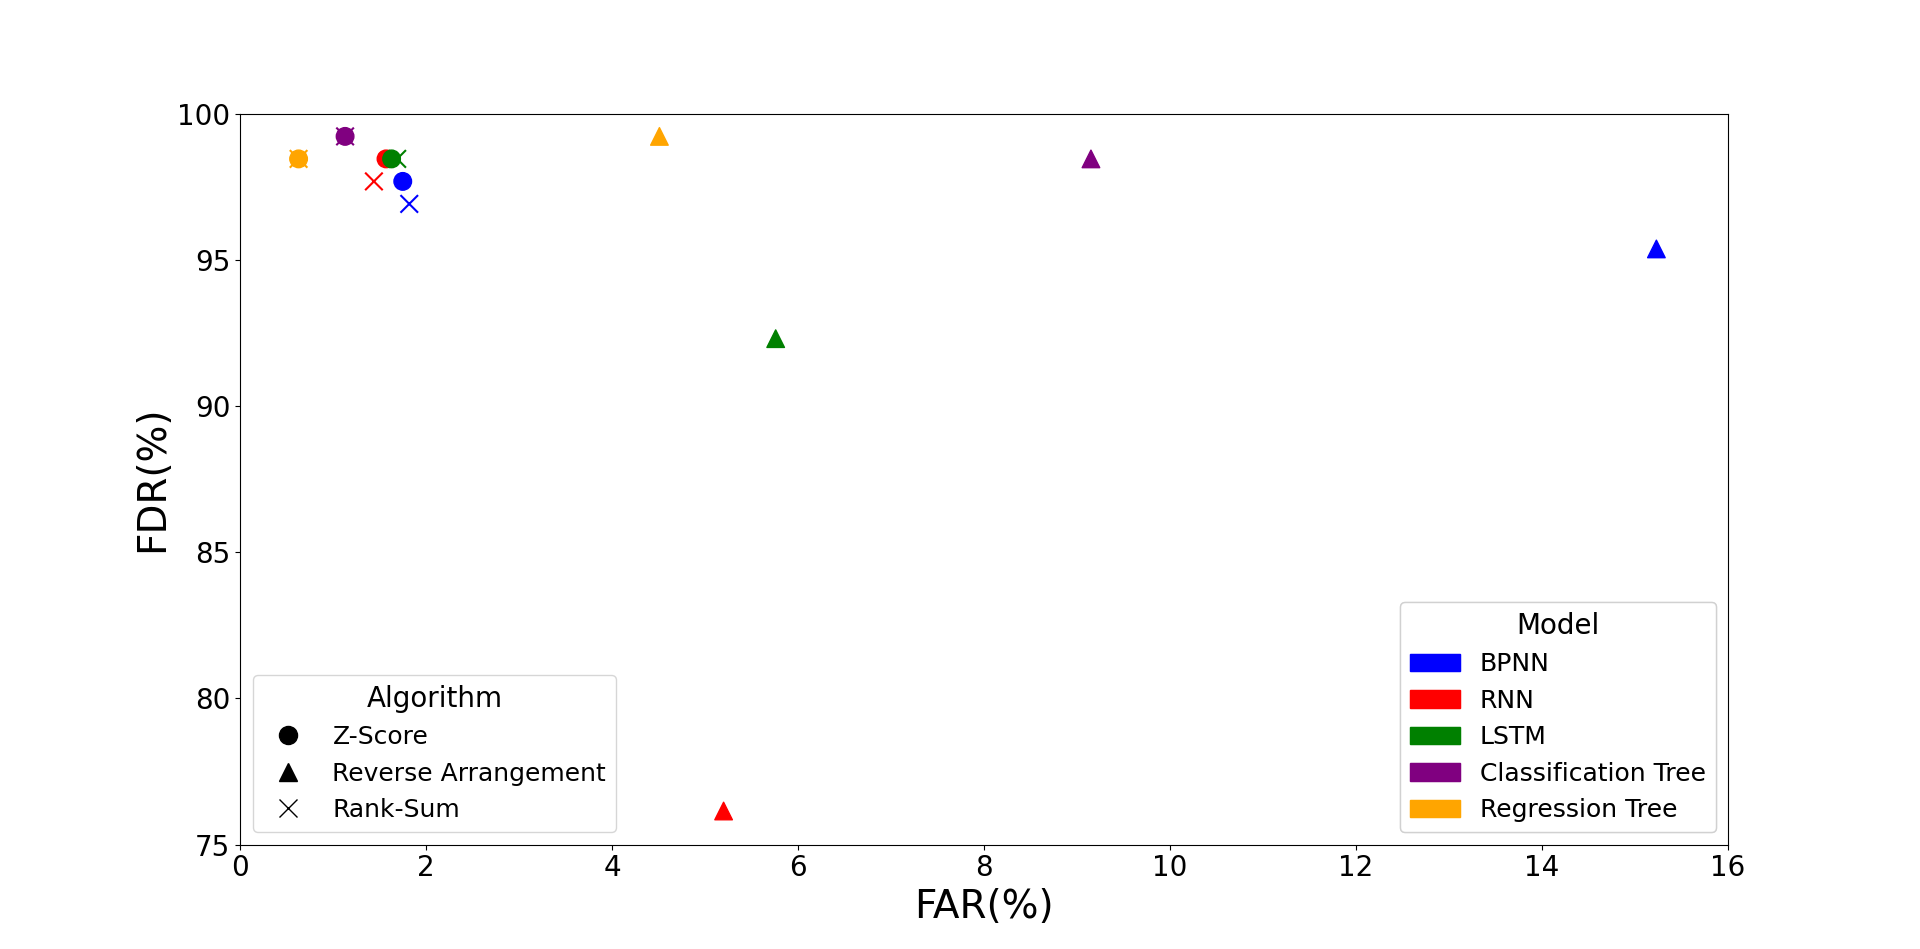
\includegraphics[width=1.0\linewidth]{FS_Binary.png}
  \caption[Feature Selection Results]{Results for different feature selection algorithms for binary models for Feature Count = 15}
  \label{fig:fs_binary}
\end{center}
\end{figure}

The most striking pattern we can observe is that the Reverse Arrangement algorithm had a worse performance than the other two on all scenarios we have tested.

Moreover, the Z-Score algorithm is slightly better than the Rank-Sum test for the network-based models.
However, the result of these two algorithms is the same for our decision trees.

If we observe which features are kept by the three algorithms, we see that 11 of them are common to all of them.
These are features such as Reallocated Sector Count, Temperature and Seek Error Rate, which is to be expected since these can easily indicate failure.

Surprisingly, between the Rank-Sum and the Reverse Arrangement algorithms, only 3 of the 15 features change, but this is already enough to generate completely different results.
Two of the features that appear in the selection done by the Reverse Arrangement but do not appear on Rank-Sum one are change rate features: the Current Pending Sector Change Rate and the Seek Error Rate Change Rate.
The third one, High Fly Writes, also do not appear in the Z-Score selection.

This indicates that the change rate features allow the models to learn the classification problem more efficiently.
We will explore this further on Subsection \ref{subsec:change_rate_impact}.

\subsection{Voting}

To observe how the voting process can influence the performance of the models, we ran our experiments with the default configuration but using 7 votes instead of only 1.
We still kept the vote threshold at 0.5.
As discussed on Subsection \ref{subsec:voting}, for the binary models we are presenting, only the Class Based Voting Algorithm can be used.

The results of this experiment are displayed on Table \ref{table:results_binary_voting}. 

\begin{table}
  \begin{center}
    \begin{tabular}{|c|c|c|c|c|}
      \hline
    Model & FAR(\%) & FDR(\%) & TIA(h) & TIA SD(h) \\
    \hline
    BPNN & 1.63 & 96.15 & 366.0 & 145.0 \\
    RNN & 1.63 & 99.23 & 375.3 & 137.7 \\
    LSTM & 1.13 & 98.46 & 362.7 & 145.6\\
    Classification Tree & 1.13 & 99.23 & 359.8 & 147.7 \\
    Regression Tree & 1.13 & 99.23 & 341.0 & 154.2 \\
    \hline
    \end{tabular}
    \caption[Results Binary Models with Voting]{Results for binary models with Vote Count set to 7}
    \label{table:results_binary_voting}
  \end{center}
\end{table}

As we can see, the results are similar to the original ones.
The FAR and the FDR of the RNN, classification and regression trees did not change at all.
The LSTM objectively improved, since it tied the lowest FAR we have found and increased its FDR compared to the case with only one vote. 

Moreover, on almost all models the TIA decreased by a relatively small amount.
This was expected due to the fact that now more than one sample is needed to classify a disk as failing, so it can be seen as more evidence that the hard drive is failing is needed before it is flagged as so.

The fact that the FDR didn't change a lot was to be expected given the results displayed on Figures \ref{fig:tia_binary_network} and \ref{fig:tia_binary_tree}.
Usually, a failing disk will start producing samples indicating it much before it crashes.

Therefore, the probability that a sequence with many samples that can be predicted as failing is high.
Thus, the decrease of the FDR is expected to be small, which is the result we obtained.

For the LSTM, we obtained a result that at first seem counterintuitive.
Even though with 7 votes more than one sample needs to be classified as failing in order to flag the disk as failing, we obtained a smaller FAR.
In other words, the number of disks flagged as failing was strictly smaller.

But this is due to the method we use to do the voting.
Since, as explained in section \ref{subsec:voting}, with more votes a longer sequence is passed to the LSTM at once, with more than one vote, it is able to apply its ability to learn sequences.
So the result we observed is actually a consequence of the capacity of the time sensitive models to take into account the context in which a sample was taken.

Now, if we keep the vote count to 7 but increase the vote threshold to 0.8, we obtain the results shown on Table \ref{table:results_binary_threshold}.

\begin{table}
  \begin{center}
    \begin{tabular}{|c|c|c|c|c|}
      \hline
    Model & FAR(\%) & FDR(\%) & TIA(h) & TIA SD(h) \\
    \hline
    BPNN & 1.63 & 96.15 & 366.0 & 145.1 \\
    RNN & 1.63 & 99.23 & 375.3 & 137.7 \\
    LSTM & 0.81 & 98.46 & 362.5 & 146.0 \\
    Classification Tree & 1.13 & 99.23 & 359.7 & 147.7 \\
    Regression Tree & 0.69 & 98.46 & 342.8 & 152.9 \\
    \hline
    \end{tabular}
    \caption[Results Binary Models with Threshold]{Results for binary models with Vote Count set to 7 and Vote Threshold equal to 0.8}
    \label{table:results_binary_threshold}
  \end{center}
\end{table}

Again we observe a further decrease on the value of the FAR, the FDR and the TIA for some models.
The regression tree is able to achieve an FAR as small as 0.69\% which is the smallest value we found for it.

The most interesting approach of using a voting algorithm is that the value of the vote count and threshold can be modified without needing to retrain the model, which is not the case when changing other hyperparameters such as the feature count or the feature selection algorithm.
Therefore, the voting method is a powerful and fast to use tool to fine tune the FAR-FDR tradeoff.

\subsection{Change Rate Impact}\label{subsec:change_rate_impact}

The next step was to observe how including the change rate of the original SMART attributes affects the performance of our models.
So, we trained our models without computing the change rates.
In order to remove any impact due to feature selection algorithms, we used all 12 SMART attributes.

The results are displayed on table \ref{table:results_binary_no_change_rate}

\begin{table}
  \begin{center}
    \begin{tabular}{|c|c|c|c|c|}
      \hline
    Model & FAR(\%) & FDR(\%) & TIA(h) & TIA SD(h) \\
    \hline
    BPNN & 2.13 & 98.46 & 363.7 & 145.1 \\
    RNN & 1.57 & 98.46 & 357.4 & 145.9 \\
    LSTM & 2.07 & 95.38 & 361.8 & 143.6 \\
    Classification Tree & 1.07 & 99.23 & 354.7 & 147.8 \\
    Regression Tree & 1.07 & 97.69 & 354.7 & 147.8 \\
    \hline
    \end{tabular}
    \caption[Results Binary Models with Voting, no Change Rate]{Results for binary models with Vote Count set to 7 without Change Rate features}
    \label{table:results_binary_no_change_rate}
  \end{center}
\end{table}

Most notably, every model had a worse performance compared to the original version using the change rates.
This shows that the change rate we computed carries information than can be used by the models to better learn the problem, both for the time sensitive and time insensitive models.

Moreover, it is interesting to see that over all the models we presented in this section, the ones that had the best performance were the two decision tree ones with information about the change rates.
The fact that they both classification and regression trees are time insensitive implies that we can encode useful information about the problem in the form of change rates. 

\section{Multiclass Models}

The next step is to investigate the behavior of the multiclass models.
Most importantly, we used as a base value a health status Count of 4.

The results of our experiment are displayed on Tables \ref{table:results_multiclass_score_one_vote} and \ref{table:results_multiclass_class_one_vote}, presenting the performance of the models when using the Score and Class Based Voting Algorithms respectively.
All experiments were performed with a health status Count of 4 and a vote count of one.

Some modification on the hyperparameters were needed when compared to the binary models.
For the regression tree, for instance, the maximum depth of the tree had to be increased to 15.

Moreover, for the RNN and the LSTM models, the number of failing samples had to be increased to 96 to obtain a better granularity of the training samples corresponding to each class.
This impacted the time required to train these models, but it was still around 40 minutes in an ordinary desktop computer's CPU, which is still manageable.

\begin{table}
  \begin{center}
    \begin{tabular}{|c|c|c|c|c|}
      \hline
    Model & FAR(\%) & FDR(\%) & TIA(h) & TIA SD(h) \\
    \hline
    BPNN & 1.63 & 95.38 & 359.3 & 144.9 \\
    RNN & 3.57 & 94.62 & 375.9 & 134.7 \\
    LSTM & 1.94 & 97.69 & 358.4 & 142.9 \\
    Classification Tree & 1.25 & 96.92 & 347.7 & 144.1 \\
    Regression Tree & 0.75 & 99.23 & 353.0 & 147.8 \\
    \hline
    \end{tabular}
    \caption[Results Multiclass Models, Score Voting, 1 vote]{Results for multiclass models with Score Based Voting(1 vote)}
    \label{table:results_multiclass_score_one_vote}
  \end{center}
\end{table}

\begin{table}
  \begin{center}
    \begin{tabular}{|c|c|c|c|c|}
      \hline
    Model & FAR(\%) & FDR(\%) & TIA(h) & TIA SD(h) \\
    \hline
    BPNN & 1.50 & 95.38 & 359.7 & 142.3 \\
    RNN & 1.32 & 96.92 & 355.1 & 145.5 \\
    LSTM & 1.88 & 97.69 & 354.2 & 146.7 \\
    Regression Tree & 1.13 & 99.23 & 346.5 & 149.1 \\
    \hline
    \end{tabular}
    \caption[Results Multiclass Models, Class Voting, 1 vote]{Results for multiclass models with Class Based Voting (1 vote)}
    \label{table:results_multiclass_class_one_vote}
  \end{center}
\end{table}

For the Score Voting, we omit the results for the classification tree model.
This is due to the fact that, for a classification tree, no score is assigned, and therefore the Score Based Voting Algorithm cannot be applied.

The results show that most multiclass models do not perform as well as their binary counterparts.
The main exception being, of course, the regression tree model with Score Based Voting which is able to keep the same FDR with a smaller FAR than its binary version.

If we compare the impact of the two voting algorithms, we observe that most models have a better performance using Class Based Voting for this scenario of using a Vote Count equal to 1.

Our results conflict with the ones presented by \cite{Xu16} which concluded beyond any doubt that multiclass RNNs are the most performant multiclass method.
This can be due multiple factors.
Firstly, the datasets are not the same, as we only have access to a subset of the dataset used in \cite{Xu16}.

Secondly, there were some models that us and them implemented.
Namely, these are the binary and multiclass BPNN as well as the classification tree.
These three models have results much closer to the ones we obtained with our multilevel RNN.


This fact indicates that we made a more unbiased fine-tuning of the hyperparameters of the models.
These results show the importance of the current work of more impartially comparing different models instead of trying to prove that a specific one performs better than others.

\subsection{Voting}

In order to evaluate our proposed voting algorithm and compare it with the other one already present in literature, we performed the experiments now using a vote count equal to 7.
The results obtained using the Score Based Voting Algorithm and the Class Based one are shown on Tables \ref{table:results_multiclass_score_multi_vote} and \ref{table:results_multiclass_class_multi_vote} respectively.

\begin{table}
  \begin{center}
    \begin{tabular}{|c|c|c|c|c|}
      \hline
    Model & FAR(\%) & FDR(\%) & TIA(h) & TIA SD(h) \\
    \hline
    BPNN & 1.57 & 95.38 & 366.3 & 142.4 \\
    RNN & 4.51 & 96.15 & 342.9 & 154.3 \\
    LSTM & 5.33 & 99.23 & 377.1 & 135.5 \\
    Regression Tree & 0.63 & 99.23 & 359.1 & 147.7 \\
    \hline
    \end{tabular}
    \caption[Results Multiclass Models, Score Voting, 7 votes]{Results for multiclass models with Score Based Voting(7 votes)}
    \label{table:results_multiclass_score_multi_vote}
  \end{center}
\end{table}

\begin{table}
  \begin{center}
    \begin{tabular}{|c|c|c|c|c|}
      \hline
    Model & FAR(\%) & FDR(\%) & TIA(h) & TIA SD(h) \\
    \hline
    BPNN & 1.50 & 95.38 & 365.7 & 142.0 \\
    RNN & 1.32 & 98.46 & 362.1 & 145.7 \\
    LSTM & 4.70 & 99.23 & 377.1 & 135.5\\
    Classification Tree & 5.33 & 99.23 & 377.1 & 135.5 \\
    Regression Tree & 0.69 & 99.23 & 359.2 & 147.4 \\
    \hline
    \end{tabular}
    \caption[Results Multiclass Models, Class Voting, 7 votes]{Results for multiclass models with Class Based Voting(7 votes)}
    \label{table:results_multiclass_class_multi_vote}
  \end{center}
\end{table}

If we compare these results with the ones in Tables \ref{table:results_multiclass_score_one_vote} and \ref{table:results_multiclass_class_one_vote} which use a vote count equal to 1, we observe different behaviors.
The BPNN kept the same FDR but obtained a smaller FAR.
The FAR when using Class Based Voting was slightly smaller.

For the LSTM and classification tree, the FDR was improved, although the FAR increased by a noticeable amount.

The RNN in particular improved the most by using the Class Based Voting.
It achieved a better FAR and FDR than either the version using one vote and the one with 7 votes and Score Based Voting.

The regression tree model was able to keep a great FDR equivalent to the best values we have obtained over all models we have presented so far.
At the same time, increasing the number of votes decreased the FAR, with our proposed Score Based Voting obtaining the smallest FAR.

\subsection{Health Status Count}

During our experiments, we noticed that increasing the number of different classed to 5 or 6 resulted in patterns that were more difficult for our models to learn.
Specially for the RNN and LSTM, the result of the experiment was highly dependent on the seed used.

This is mainly due to the fact that when increasing the health status count there are two possible scenarios.
The first is that we decrease the number of samples per class.
The other option is to increase the Number of Failing Samples to mitigate the effect of the decrease of samples per class, which results in the training set having less relevant samples since they will be taken far away from the critical moment of failure.

Either way, it may make it more difficult for our models to learn to predict failures.
Indeed, we observe that for a health status count of 3 or 4, our models are still able to perform well.
On the other hand, for a higher number of classes, the effects mentioned on the last paragraph override the benefits we gain by interpreting the problem from a multiclass point of view.

This implies that the models' performance are highly sensitive to the value of health status count.
However, given that the ideal value is a small integer number, it is not very difficult to explore the space of possibilities to find the best one.

On Tables \ref{table:results_multiclass_three_health_status_score_voting} and \ref{table:results_multiclass_three_health_status_class_voting} we display the results of our experiments when Health Status Count is set to 3 and with Score Based and Class Based Voting respectively.

\begin{table}
  \begin{center}
    \begin{tabular}{|c|c|c|c|c|}
      \hline
    Model & FAR(\%) & FDR(\%) & TIA(h) & TIA SD(h) \\
    \hline
    BPNN & 1.69 & 96.92 & 358.6 & 144.5 \\
    RNN & 1.32 & 98.46 & 368.3 & 138.6 \\ 
    LSTM & 1.82 & 98.46 & 356.1 & 142.9\\
    Regression Tree & 1.63 & 97.69 & 350.3 & 146.6 \\
    \hline
    \end{tabular}
    \caption[Results Multiclass Models with Health Status Count set to 3, Score Voting]{Results for Multiclass Models with Health Status Count set to 3 using Score Based Voting}
    \label{table:results_multiclass_three_health_status_score_voting}
  \end{center}
\end{table}

\begin{table}
  \begin{center}
    \begin{tabular}{|c|c|c|c|c|}
      \hline
    Model & FAR(\%) & FDR(\%) & TIA(h) & TIA SD(h) \\
    \hline
    BPNN & 1.69 & 96.92 & 358.6 & 144.5 \\
    RNN & 2.57 & 95.38 & 369.3 & 136.0 \\ 
    LSTM & 1.82 & 98.46 & 356.1 & 142.9\\
    Classification Tree & 1.57 & 96.92 & 352.4 & 139.3 \\
    Regression Tree & 1.25 & 100.00 & 367.4 & 140.5 \\
    \hline
    \end{tabular}
    \caption[Results Multiclass Models with Health Status Count set to 3, Class Voting]{Results for Multiclass Models with Health Status Count set to 3 using Class Based Voting}
    \label{table:results_multiclass_three_health_status_class_voting}
  \end{center}
\end{table}

For the network based models with score based voting, reducing the health status count from 4 to 3 resulted in an improvement.
In the case of the RNN specifically, it achieved a FAR smaller than its binary counterpart, with the tradeoff being a slight worse FDR that is still acceptably high.

If we directly compare the impact of each voting algorithm we see that the network based models perform consistently better when using our proposed score based voting system.

On the other hand, one of the most striking results we have obtained during this research is the regression tree that obtained a 100\% failure detection rate while keeping a small FAR.
In all published research we have found only one other model who reached an FDR of 100\%: the binary BPNN published in \cite{Zhu13}, which had an FAR of 2.26\%.
However, our regression tree did so while cutting the FAR in half.

This is strong evidence of the power of our approach to modify the labeling of the samples to take into account their proximity to the moment of failure.
Therefore, the health status method can bring a significant improvement to the solution of the hard drive failure prediction problem.